Let's suppose that we somehow know $p(x)$. We need to sample from this distribution. We can use the following algorithm:

\begin{equation*}
    x^{m+1} = x^m + \frac{x}{2} \underbrace{\frac{\partial}{\partial x} \log p(x^{(m)})}_{\text{Score function}} + \sqrt{x} \varepsilon, \quad \varepsilon \sim \mathcal{N}(0, 1).
\end{equation*}

And suppose that we could build a series of distributions: 

\[ 
    p_0(x) \to p_1(x) \to \ldots \to p_T(x),
\]

where the first is Data distribution, the last one is is Standart Gaussian. Each of the distributions is <<close>> to the previous one. We can use the following algorithm to sample from the last distribution: 

\begin{algorithm}
    \caption{Sampling}
    \begin{algorithmic}
        \For {$t = T - 1, \ldots, 0$}
            \State $x_t^{(0)} = x_{t+1}^{(M)}$
            \For {$m = 1, \ldots, M$}
                \State $x_{t}^{(m)} = x_{t}^{(m-1)} + \frac{\partial}{\partial x} \log p_t(x_{t}^{(m-1)}) + \sqrt{x_{t}^{(m-1)}} \varepsilon, \quad \varepsilon \sim \mathcal{N}(0, 1)$
            \EndFor
        \EndFor
        \State $X_0^{(M)}$
    \end{algorithmic}
\end{algorithm}

As a constructive way we can take 
\[ 
    x_0 \sim p_0(x) \to x_1 \to \ldots \to x_T,
\]

where 

\begin{equation*}
    \begin{aligned}
        x_t &= \sqrt{1 - \beta} x_{t - 1} + \sqrt{\beta} \varepsilon, \quad \varepsilon \sim \mathcal{N}(0, 1), \quad \beta \ll 1; \\ 
        x_t &= \sqrt{\overline{\alpha_t}} x_0 + \sqrt{1 - \overline{\alpha_t}} \varepsilon, \quad \varepsilon \sim \mathcal{N}(0, 1), \quad \overline{\alpha_t} = (1 - \beta)^t,
    \end{aligned}
\end{equation*}

and in this scheme at sufficiently large $T$ we will obtain $p_T(x_T) = \mathcal{N}(0, 1)$, since $\overline{\alpha_t} \approx 0$. \\ 

Now let's assume $$s_\theta (x_t, t) \approx \frac{\partial}{\partial x} \log p_t (x_t),$$ for which we can write 

\begin{equation*}
    \begin{aligned}
        \int || s_\theta (x_t, t) &-\frac{\partial}{\partial x} \log p_t (x_t) ||^2 p_t(x_t) dx_t \\ 
        &= \int p_t(x) \left[ s_\theta^T (x, t) s_\theta (x, t) - 2 s_\theta^T (x, t) \frac{\partial}{\partial x} \log p_t (x) + \frac{\partial}{\partial x} \log p_t (x) \frac{\partial}{\partial x} \log p_t (x) \right] dx \\ 
        &= \int p_t(x) s_\theta^T (x, t) s_\theta (x, t) dx - 2 \int p_t(x) s_\theta^T (x, t) \frac{\partial}{\partial x} \log p_t (x) dx + \Const \\ 
        &= \int p_t(x) s_\theta^T (x, t) s_\theta (x, t) dx - 2 \int s_\theta^T (x, t) \frac{\partial}{\partial x} p_t(x) dx + \Const \\ 
        &\qquad \qquad \qquad\left\{ p_t(x) = \int q(x | x_0) p_o (x_0) dx_0 \right\} \\ 
    \end{aligned}
\end{equation*}

\begin{equation*}
    \begin{aligned}
        &= \iint q(x | x_0) p_0 (x_0) s_\theta^T (x, t) s_\theta (x, t) d x_0 dx - 2 \iint p_0(x_0) s_\theta^T (x, t) \frac{\partial}{\partial x} q(x | x_0) d x d x_0 + \Const \\ 
        &\qquad \qquad \qquad \left\{ \frac{\partial}{\partial x} q(x | x_0) = q(x | x_0) \frac{\partial}{\partial x} \log q(x | x_0) \right\} \\ 
        &= \iint q( x | x_0) p_0 (x_0) s_\theta^T (x, t) s_\theta (x, t) d x d x_0 - 2 \iint p_0(x_0) s_\theta^T (x, t) q(x | x_0) \frac{\partial}{\partial x} \log q(x | x_0) d x d x_0 + \Const \\
        &= \iint q( x | x_0) p_0 (x_0) || s_\theta (x, t) - \frac{\partial}{\partial x} \log q(x | x_0) ||^2 d x d x_0 + \Const
    \end{aligned}
\end{equation*}

So how do we train our model? Let's firstly name the following:
\[ 
    \underbrace{x_0}_{\text{observed}} \to \underbrace{x_1 \to \ldots \to x_t \to \ldots \to x_T}_{\text{latent}},
\]
And now proceed to lower bound:

\begin{equation*}
    \begin{aligned}
        \log p_\theta(x_0) &\geq \int q(x_1, \ldots, x_T | x_0) \log \frac{p_\theta(x_0, \ldots, x_T)}{q(x_1, \ldots, x_T | x_0)} d x_1 \ldots d x_T \\
        &= \int q(x_1 | x_0) q (x_2 | x_1) \ldots q(x_T | x_{T-1}) \log \frac{p^\theta_T(x_T) p^\theta_{T-1}(x_{T-1} | x_T) \ldots p^\theta_1(x_1 | x_0)}{q(x_1 | x_0) q(x_2 | x_1) \ldots q(x_T | x_{T-1})} d x_1 \ldots d x_T \\
        &\qquad \qquad \qquad\left\{ q(x_{t - 1} | x_t, x_0) = \MN (x_{t - 1} | \widetilde{\mu_{t - 1}}, \widetilde{\beta_{t - 1}}) = \frac{q(x_t | x_{t - 1}) q(x_{t - 1} | x_0)}{q(x_t | x_0)} \right\} \\ 
        &= \int q(x_1, \ldots, x_T | x_0) \log \frac{p^\theta_T(x_T) p^\theta_{T-1}(x_{T-1} | x_T) \ldots p^\theta_1(x_1 | x_0)}{q(x_T | x_0) q(x_{T-1} | x_T, x_0) \ldots q(x_1 | x_2, x_0)} d x_1 \ldots d x_T \\
        &= \int q(x_1 | x_0) \log p^\theta_0 (x_0 | x_1) d x_1 + \underbrace{\int q(x_T | x_0) \log \frac{p^\theta_T(x_T)}{q(x_T | x_0)} d x_T}_{0} + \\ 
        &\qquad \qquad \qquad+\sum_{t = 2}^T \int q(x_t | x_0) q(x_{t - 1} | x_t, x_0) \log \frac{q(x_{t - 1} | x_t, x_0)}{p^\theta(x_{t - 1} | x_t, x_0)} d x_{t - 1} d x_t \\
        &= \underbrace{\int q(x_1 | x_0) \log p^\theta_0 (x_0 | x_1) d x_1}_{\Const} - \sum_{t = 2}^T \int q(x_t | x_0) \operatorname{KL} (q(x_{t - 1} | x_t, x_0) || p^\theta(x_{t - 1} | x_t)) d x_{t - 1} d x_t \\ 
        &\qquad \qquad \qquad \qquad \qquad \qquad\to \max_{\theta}
    \end{aligned}
\end{equation*}

We may estimate 
\[ 
    q(x_{t - 1} | x_t, x_0) = \MN (x_{t - 1} | \widetilde{\mu_{t - 1}}, \widetilde{\beta_{t - 1}}) = \frac{q(x_t | x_{t - 1}) q(x_{t - 1} | x_0)}{q(x_t | x_0)},
\]
where 
\[ 
    \widetilde{\mu_{t - 1}(x_t, x_0)} = \frac{\sqrt{\overline{\alpha_{t - 1}}} \beta}{1 - \overline{\alpha_{t}}} x_0 + \frac{\sqrt{1 - \beta}(1 - \overline{\alpha_{t - 1}})}{1 - \overline{\alpha_t}}x_t,
\] 
which indeed meant that $x_{t-1}$ is a linear combination of $x_t$ and $x_0$ and it lies somewhere around thie estimated mean with some Gaussian variable. On the illustration below you can see the scheme of the model. \\ 

\begin{figure}[htb]
    \centering
    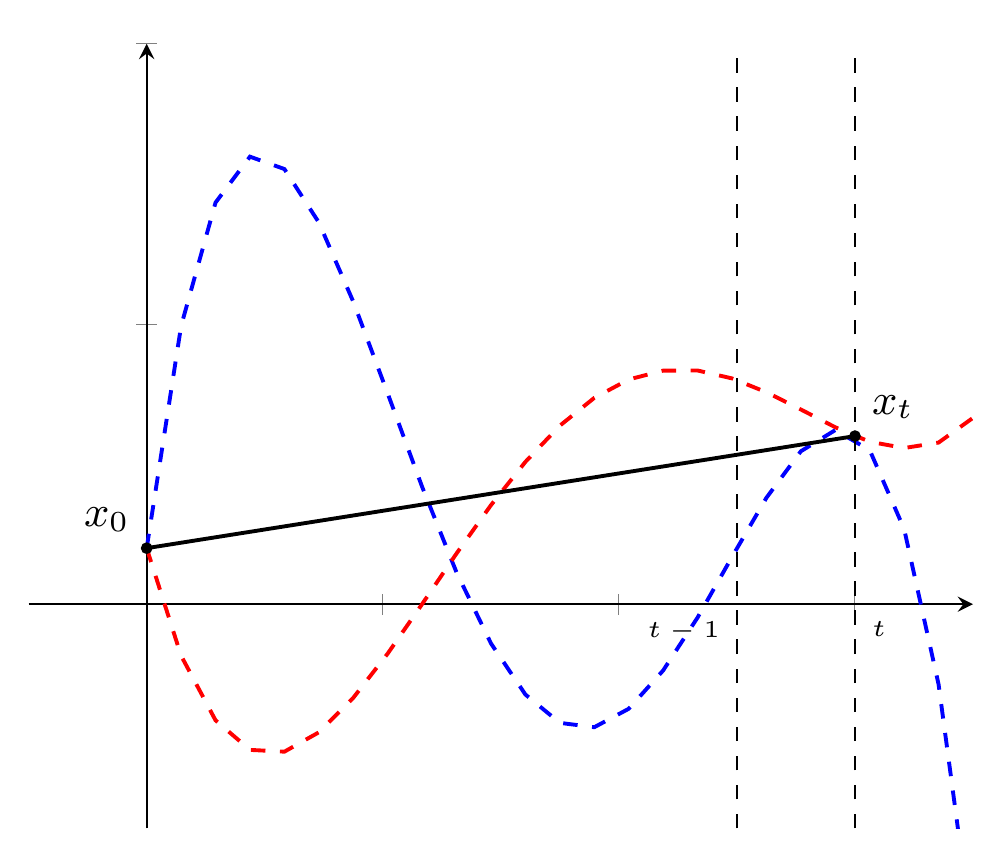
\begin{tikzpicture}[scale=1.75]
        \begin{axis}[
            axis lines=middle,
            %xlabel=$t$, ylabel=$x$,
            xmin=-1, xmax=7,
            ymin=-4, ymax=10,
            xticklabels={},
            yticklabels={},
        ]

        \addplot[dashed, blue, thick, domain=0:7] {1 + (205*x)/12 - (307*x*x)/24 + (35*x*x*x)/12 - (5*x*x*x*x)/24};
        \addplot[dashed, red, thick, domain=0:7] {1 - (121*x)/15 + (27*x*x)/5 - (16*x*x*x)/15 + (x*x*x*x)/15};
        \draw [black, dashed] (axis cs: 5, -4) -- (axis cs: 5,10);
        \draw [black, dashed] (axis cs: 6, -4) -- (axis cs: 6,10);
        \draw [black, thick] (axis cs: 0, 1) -- (axis cs: 6,3);

        \addplot[mark size=1pt, only marks,mark=*,mark options={fill=black}] coordinates {(0,1)} node[above left,font=\small] {$x_0$};
        \addplot[mark size=1pt, only marks,mark=*,mark options={fill=black}] coordinates {(6,3)} node[above right,font=\small] {$x_t$};
        \addplot[mark options={fill=black}] coordinates {(6,0)} node[below right,font=\tiny] {$t$};
        \addplot[mark size=1pt, mark options={fill=black}] coordinates {(5,0)} node[below left,font=\tiny] {$t-1$};

        \end{axis}
    \end{tikzpicture}
    \caption{Two pathes of points from $x_0$ to $x_t$ and estimation of $x_{t-1}$.}
\end{figure}

We know, how to compute $q(x_{t-1} | x_t, x_0)$, so we can define 

\begin{equation*}
    \begin{aligned}
        p^\theta(x_{t-1} | x_t) = q(x_{t - 1} | x_t, \widehat{x_\theta} (x_t, t))
    \end{aligned}
\end{equation*}

$x_\theta$ is a neural network, which will be trained. And the criterion comes as 

\begin{equation*}
    \begin{aligned}
        \operatorname{KL} (q(x_{t - 1} | x_t, x_0) || p^\theta(x_{t - 1} | x_t)) &= \Const + Const' || \widetilde{\mu_{t-1}} - \mu_0 ||^2 \\ 
        &= \Const + \Const'' || x_0 - x_\theta(x_t, t) ||^2 \to \min_{\theta} \\ 
        &\Leftrightarrow \Const + \Const''' || \varepsilon - \varepsilon_\theta(x_t, t) ||^2 \to \min_{\theta} 
    \end{aligned}
\end{equation*}

with
\begin{equation*}
    x_\theta (x_t, t) = \frac{x_t - \sqrt{1 - \overline{\alpha_t}} \varepsilon_\theta(x_t, t)}{\sqrt{\overline{\alpha_t}}}, \quad x_0 = \frac{x_t - \sqrt{1 - \overline{\alpha_t}} \varepsilon}{\sqrt{\overline{\alpha_t}}}, \quad \text{and} \quad s_\theta(x, t) = \frac{- \varepsilon_\theta(x, t)}{\sqrt{1 - \overline{\alpha_t}}}.
\end{equation*}

And the generation process looks like 
\begin{algorithm}
    \caption{Generation}
    \begin{algorithmic}
        \State \textbf{Initialise} $x_T \sim \mathcal{N}(x_T | 0, I) = p(x_T)$ 
        \For {$t = T - 1, \ldots, 0$}
            \State $x_{t - 1} \sim p(x_{t - 1} | x_t, \theta) = q(x_{t - 1} | x_t, x_\theta(x_t, t)) = \mathcal{N}(x_{t - 1} | \mu(x_t, x_\theta(x_t, t)), \widetilde{\beta_{t}} I)$
        \EndFor
        \State \textbf{Obtain} $x_0 \sim p(x_0 | x_1) = \mathcal{N}(x_0 | x_1, s I) \quad \text{where} \quad s \ll 1$
    \end{algorithmic}
\end{algorithm}
